\documentclass[10pt, letterpaper]{article}

% Packages:
\usepackage[
    ignoreheadfoot,
    top=2 cm,
    bottom=2 cm,
    left=2 cm,
    right=2 cm,
    footskip=1.0 cm,
]{geometry}
\usepackage[explicit]{titlesec}
\usepackage{tabularx}
\usepackage{array}
\usepackage[dvipsnames]{xcolor}
\definecolor{primaryColor}{RGB}{0, 79, 144}
\usepackage{enumitem}
\usepackage{fontawesome5}
\usepackage{graphicx}
\usepackage{amsmath}
\usepackage[
    pdftitle={CV di Leonardo Silvagni},
    pdfauthor={Leonardo Silvagni},
    pdfcreator={LaTeX},
    colorlinks=true,
    urlcolor=black
]{hyperref}
\usepackage[pscoord]{eso-pic}
\usepackage{calc}
\usepackage{bookmark}
\usepackage{lastpage}
\usepackage{changepage}
\usepackage{paracol}
\usepackage{ifthen}
\usepackage{needspace}
\usepackage{iftex}
\usepackage{verbatim}
\usepackage{etoolbox}

\ifPDFTeX
    \input{glyphtounicode}
    \pdfgentounicode=1
    \usepackage[T1]{fontenc}
    \usepackage[utf8]{inputenc}
    \usepackage{lmodern}
\fi

\usepackage[default, type1]{sourcesanspro}

% Footer style:
\AtBeginEnvironment{adjustwidth}{\partopsep0pt}
\pagestyle{empty}
\setcounter{secnumdepth}{0}
\setlength{\parindent}{0pt}
\setlength{\topskip}{0pt}
\setlength{\columnsep}{0.15cm}
\makeatletter
\let\ps@customFooterStyle\ps@plain
\patchcmd{\ps@customFooterStyle}{\thepage}{
    \color{gray}\textit{\small Leonardo Silvagni - Pagina \thepage{} di \pageref*{LastPage}}
}{}{}
\makeatother
\pagestyle{customFooterStyle}

% Section title format:
\titleformat{\section}{
    \needspace{4\baselineskip}
    \Large\color{primaryColor}
}{}{0pt}{
    \textbf{#1}\hspace{0.15cm}\titlerule[0.8pt]\hspace{-0.1cm}
}[]
\titlespacing{\section}{-1pt}{0.3cm}{0.2cm}

% List environments:
\newenvironment{highlights}{
    \begin{itemize}[
        topsep=0.10 cm,
        parsep=0.10 cm,
        partopsep=0pt,
        itemsep=0pt,
        leftmargin=0.4 cm + 10pt
    ]
}{
    \end{itemize}
}
\newenvironment{highlightsforbulletentries}{
    \begin{itemize}[
        topsep=0.10 cm,
        parsep=0.10 cm,
        partopsep=0pt,
        itemsep=0pt,
        leftmargin=10pt
    ]
}{
    \end{itemize}
}

\newenvironment{onecolentry}{
    \begin{adjustwidth}{0.2 cm + 0.00001 cm}{0.2 cm + 0.00001 cm}
}{
    \end{adjustwidth}
}

\newenvironment{twocolentry}[2][]{
    \onecolentry
    \def\secondColumn{#2}
    \setcolumnwidth{\fill, 4.5 cm}
    \begin{paracol}{2}
}{
    \switchcolumn \raggedleft \secondColumn
    \end{paracol}
    \endonecolentry
}

\newenvironment{threecolentry}[3][]{
    \onecolentry
    \def\thirdColumn{#3}
    \setcolumnwidth{1 cm, \fill, 4.5 cm}
    \begin{paracol}{3}
    {\raggedright #2} \switchcolumn
}{
    \switchcolumn \raggedleft \thirdColumn
    \end{paracol}
    \endonecolentry
}

% --- header environment ---
\newenvironment{header}{%
  \vspace*{-0.6cm}%
  \color{primaryColor}\linespread{1.3}%
  % left: photo
  \begin{minipage}[t]{3cm}%
  \vspace{-15pt}
    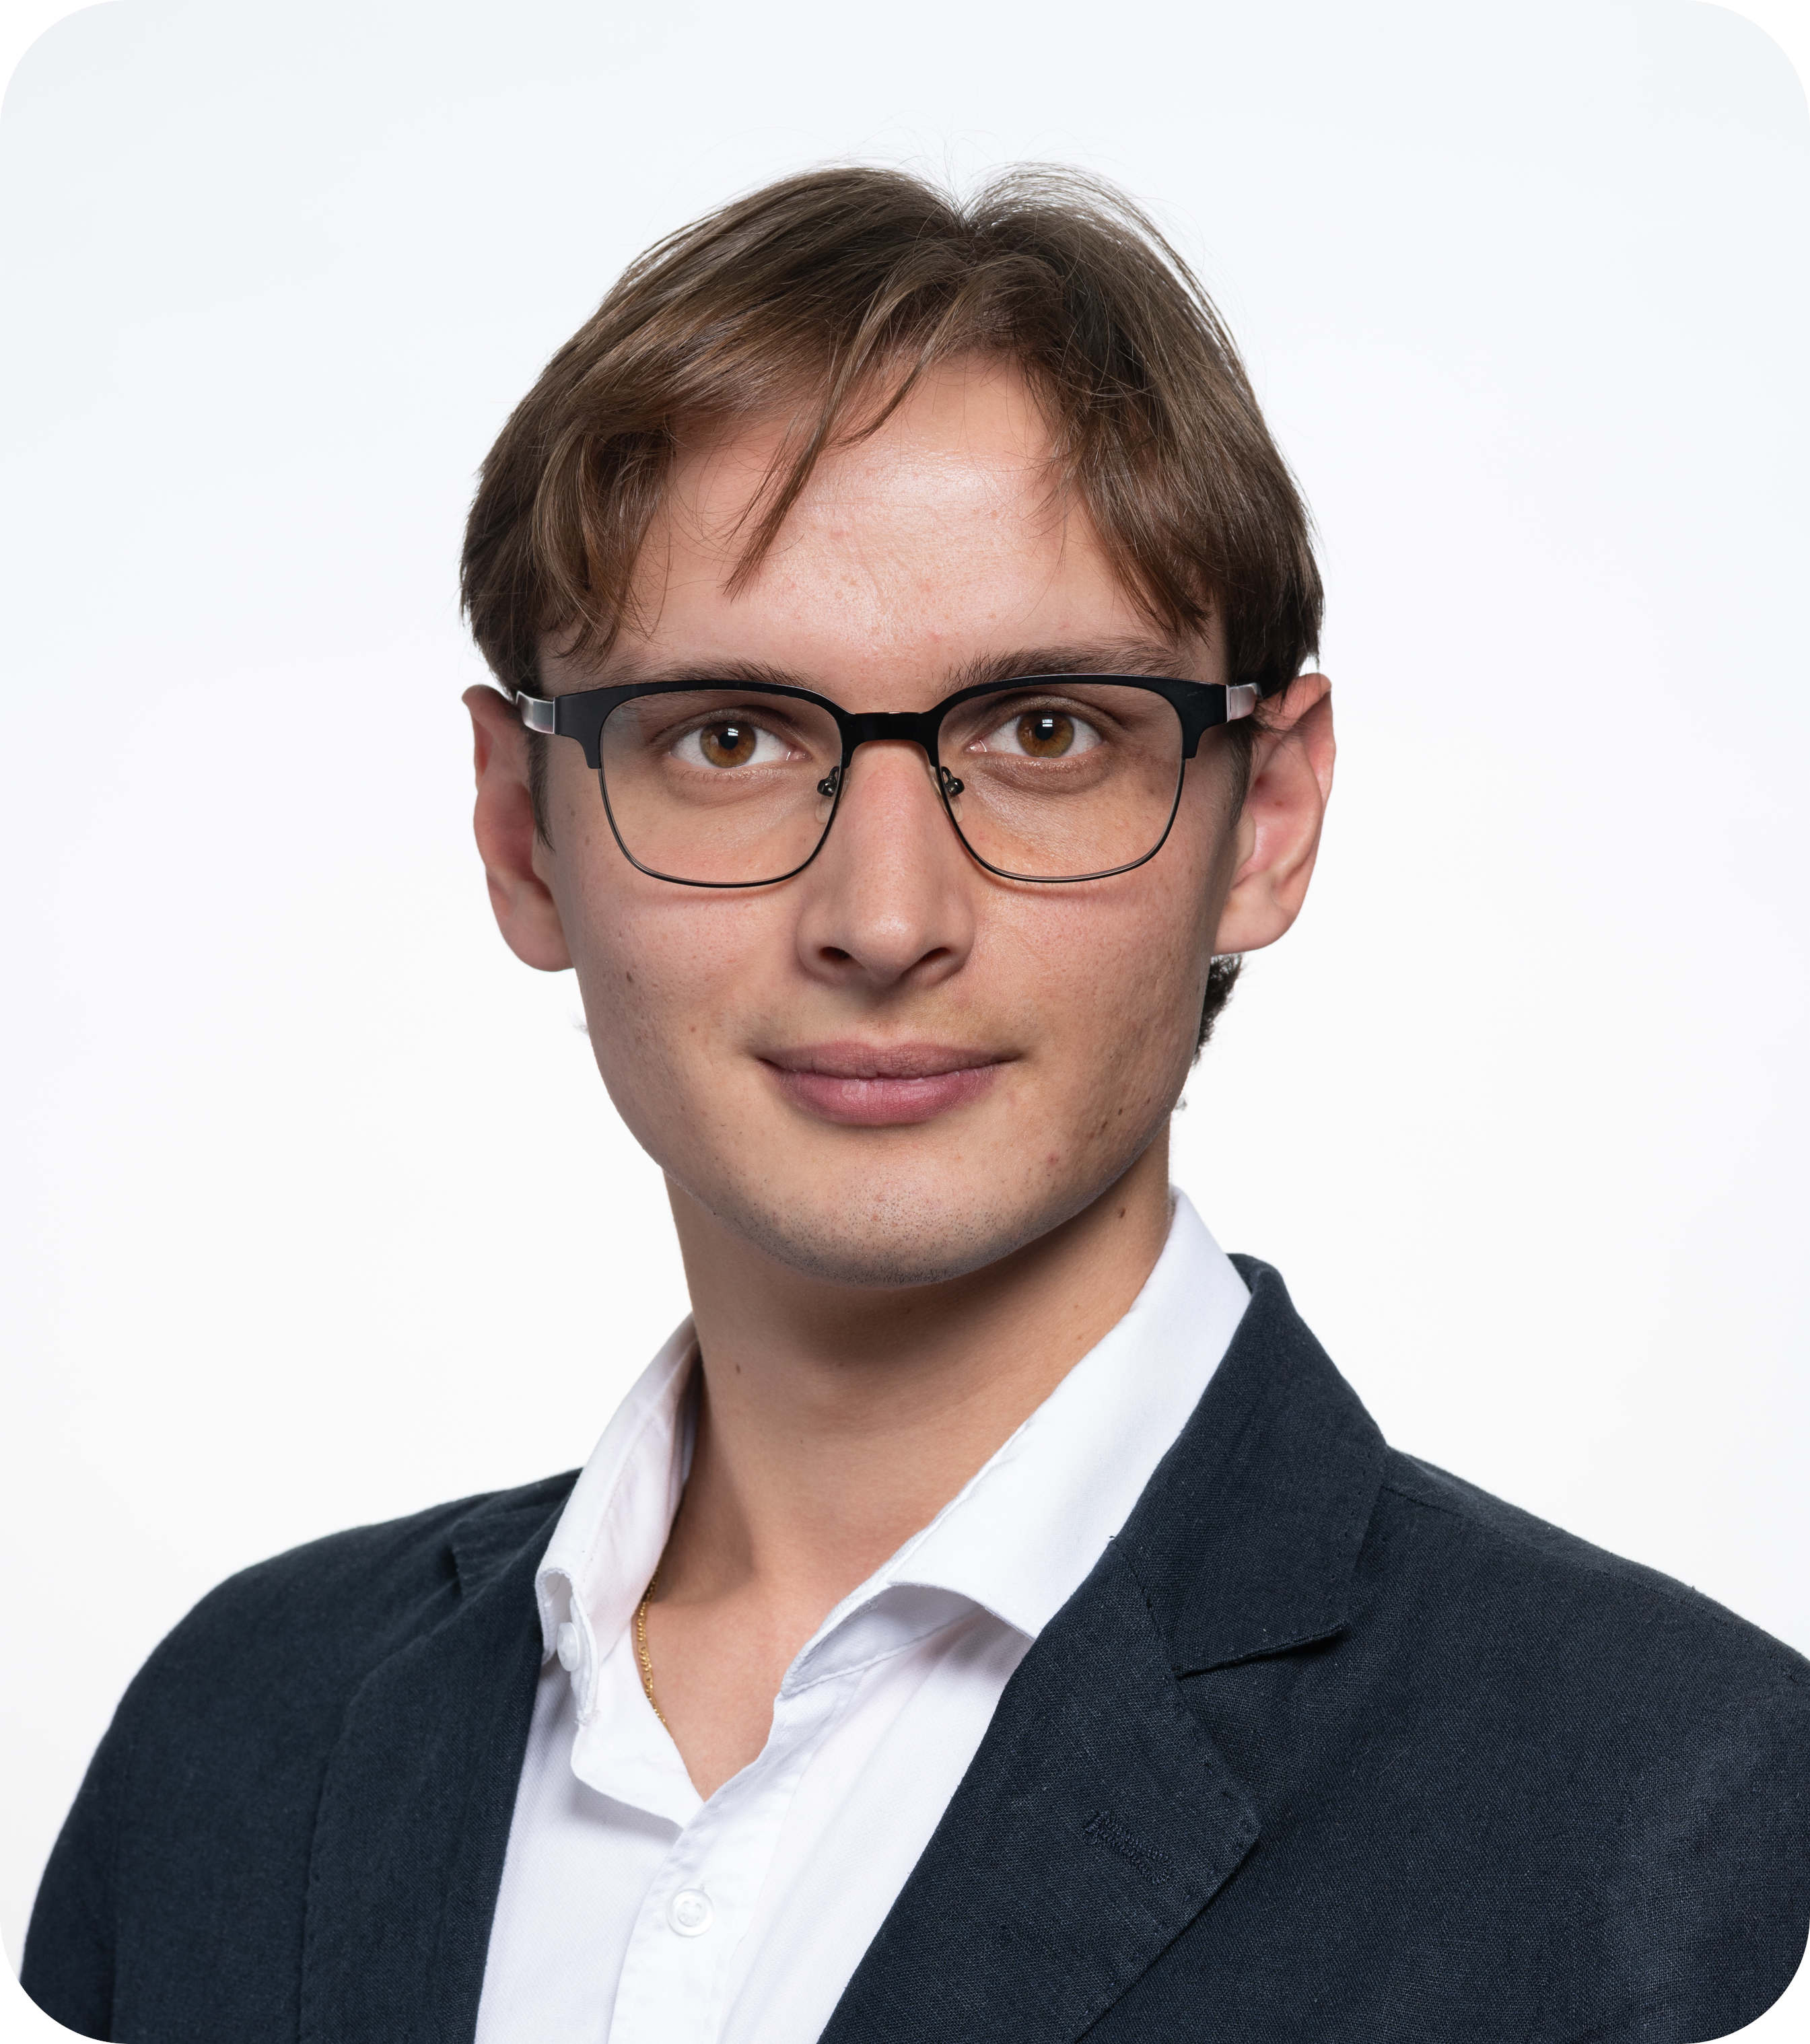
\includegraphics[width=\linewidth,keepaspectratio]{SquareLeoRound.jpg}%
  \end{minipage}%
  \hspace{1cm}
  % right: text block
  \begin{minipage}[t]{\dimexpr\linewidth-3cm-0.8em\relax}%
    \vspace{0pt}%
}{%
  \end{minipage}%
  \vspace*{-0.2cm}%
}

% Last‐updated text
\newcommand{\placelastupdatedtext}{%
  \AddToShipoutPictureFG*{%
    \put(
        \LenToUnit{\paperwidth-2 cm-0.2 cm+0.05cm},
        \LenToUnit{\paperheight-1.0 cm}
    ){\vtop{{\null}\makebox[0pt][c]{
        \small\color{gray}\textit{Ultimo aggiornamento aprile 2025}\hspace{\widthof{Ultimo aggiornamento aprile 2025}}
    }}}%
  }%
}

% Link arrow
\let\hrefWithoutArrow\href
\renewcommand{\href}[2]{%
  \hrefWithoutArrow{#1}{\ifthenelse{\equal{#2}{}}{}{#2 }\raisebox{.15ex}{\footnotesize \faExternalLink*}}%
}

\begin{document}
    \newcommand{\AND}{\unskip
        \cleaders\copy\ANDbox\hskip\wd\ANDbox
        \ignorespaces
    }
    \newsavebox\ANDbox
    \sbox\ANDbox{}

    %\placelastupdatedtext
    \begin{header}
        \fontsize{30 pt}{30 pt}\textnormal{Leonardo Silvagni}
        \vspace{0.1 cm}

        \fontsize{16 pt}{16 pt}\textnormal{Studente di Neuroingegneria all'EPFL}
        
        \normalsize
        \vspace{0.1cm}
        \mbox{{\footnotesize\faMapMarker*}\hspace*{0.13cm}1023, Crissier, Svizzera}%
        \kern 0.25 cm\AND%
        \mbox{\hrefWithoutArrow{mailto:leonardo.silvagni@gmail.com}{{\footnotesize\faEnvelope[regular]}\hspace*{0.13cm}leonardo.silvagni@gmail.com}}%
        \kern 0.25 cm\AND%
        \mbox{\hrefWithoutArrow{tel:+41783169108}{{\footnotesize\faPhone*}\hspace*{0.13cm}+41 78 316 9108}}%
        \kern 0.25 cm\AND%
        \mbox{\hrefWithoutArrow{https://www.linkedin.com/in/leonardo-silvagni}{{\footnotesize\faLinkedinIn}\hspace*{0.13cm}linkedin.com/in/leonardo-silvagni}}%
    \end{header}

    \vspace{0.1 cm}

    \section{Profilo}
    \begin{onecolentry}
        \textbf{Punti di forza:} Elaborazione dei segnali, Apprendimento automatico, Elettronica.\\
        % Ingegnere biomedico di formazione, interessato all'interfacciamento con il sistema nervoso.
        % Esperienza in manipolazione dati, analisi statistica e machine learning. Padronanza di Python, R, Matlab, C/C++; strumenti: Torch, Pandas, Numpy, Scipy, git, LaTeX; elaborazione di segnali e immagini, computer vision, dati neurali (EEG, EMG, fMRI).
    \end{onecolentry}

    \section{Formazione}

    \begin{threecolentry}{\textbf{MSc}}{2024--Presente}{\textbf{EPFL École Polytechnique Fédérale de Lausanne}, Neuroingegneria}
    \end{threecolentry}
    \vspace{0.2 cm}
    \begin{threecolentry}{\textbf{BSc}}{2024}{\textbf{ETSIT, Universidad Politécnica de Madrid}, Ingegneria Biomedica (Erasmus)}
    \end{threecolentry}
    \vspace{0.2 cm}
    \begin{threecolentry}{\textbf{BSc}}{2021--2024}{\textbf{Università di Padova}, Ingegneria Biomedica\\Voto finale: 110 e lode / 110}
    \end{threecolentry}

    \section{Progetti e Ricerca}

    \begin{twocolentry}{2025\\Progetto personale}
        \textbf{Sistema aptico di guida del passo per il rilevamento ostacoli tramite visione stereo e sensori inerziali (in corso)}
        \begin{highlights}
            \item Focus: algoritmi di visione artificiale embedded, fusione sensoriale (IMU e telecamere), ottimizzazione energetica.
        \end{highlights}
    \end{twocolentry}
    
    \begin{twocolentry}{2025\\EPFL, Losanna, CH}
        \textbf{Transistore a gate esteso per applicazioni di biosensing (in corso)}
        \begin{highlights}
            \item Ridisegno (CAD) del layout precedente con riduzione della capacità parassita del 45\% per migliorare il limite di rilevazione.
            \item Fabbricazione e test dei dispositivi (cleanroom e laboratorio umido/secco).
        \end{highlights}
    \end{twocolentry}

    \vspace{0.2 cm}
    \begin{twocolentry}{2024\\EPFL, Losanna, CH}
        \href{https://github.com/fedemengo/CS-433-ML4S}{\textbf{Machine Learning: Predizione dei compiti a partire da dati fMRI}}
        \begin{highlights}
            \item Sviluppo e validazione di modelli RNN per deconvolvere i time-course dei paradigmi di task da dati di neuroimmagine (fMRI) del dataset \textit{task-based} dell'Human Connectome Project.
        \end{highlights}
    \end{twocolentry}

    \vspace{0.2 cm}
    \begin{twocolentry}{2024\\ETSIT, Madrid, ES}
        \textbf{Saturimetro ossimetrico basato su ESP32}
        \begin{highlights}
            \item Implementazione di elaborazione del segnale in tempo reale su embedded per estrarre frequenza cardiaca e saturazione di ossigeno dal segnale PPG.
        \end{highlights}
    \end{twocolentry}

    \vspace{0.2cm}
    \begin{twocolentry}{2023--2024\\UNIPD, Padova, IT}
        \href{https://hdl.handle.net/20.500.12608/68828}{\textbf{Modelli Bayesiani dinamici della progressione nella Sclerosi Laterale Amiotrofica}}
        \begin{highlights}
            \item Validazione di un modello esistente nell'ambito dell'\textit{Explainable AI} per dati clinici, usando \textit{Dynamic Bayesian Networks}.
        \end{highlights}
    \end{twocolentry}

    \section{Competenze Tecniche}
    \begin{onecolentry}
      \textbf{Linguaggi di programmazione:} Python, R, Matlab, C/C++, LaTeX
    \end{onecolentry}
    \vspace{0.1 cm}
    \begin{onecolentry}
      \textbf{Strumenti:} git, Torch, Pandas, Numpy, Scipy, OpenCV, Scikit-learn
    \end{onecolentry} 
    \vspace{0.1 cm}
    \begin{onecolentry}
      \textbf{Competenze:} Machine Learning, Elettronica, CAD, Elaborazione di segnali e immagini, FEM/COMSOL, Computer Vision, Microfabbricazione, Analisi statistica
    \end{onecolentry} 

    \section{Esperienze Professionali}

    \begin{twocolentry}{
        Arzignano (VI), IT

2018--2020
    }
        \textbf{Docente di Elettronica}, Biblioteca \textit{Giulio Bedeschi}
        \begin{highlights}
            \item Corsi introduttivi su piattaforma Arduino ed elettronica di base per 20 studenti (13--18 anni).
            \item Tutoraggio di 25 studenti (12--16 anni) in sfide di robotica per la First Lego League. Team 4\textsuperscript{o} a livello nazionale.
        \end{highlights}
    \end{twocolentry}

    \vspace{0.2 cm}
    \begin{twocolentry}{
        Padova, IT

2021--2024
    }
        \textbf{Tutor e assistente didattico}, Università di Padova
        \begin{highlights}
            \item Tutoraggio tra pari nei corsi di \textit{Controlli automatici, Elettronica, Algebra lineare, Fisica (classica ed elettromagnetismo), Analisi I \& II}.
        \end{highlights}
    \end{twocolentry}

    \section{Organizzazioni}

    \begin{twocolentry}
        {2024--2025}{\textbf{Lead The Future Mentorship}\\
        Programma di mentorship per studenti STEM italiani.}
    \end{twocolentry}

    \vspace{0.1 cm}

    \begin{twocolentry}
        {2023}{\textbf{Bioleap}, Nucleate Italy\\
        Programma informativo di 4 mesi su medtech e startup.}
    \end{twocolentry}

    \section{Riconoscimenti \& Premi}

    \begin{threecolentry}
        {2025}{Harvard, Boston, USA}{\textbf{Bertarelli Harvard EPFL Fellowship}\\
        Borsa di studio da 120\,000 \$ (75\,000 \$ tasse universitarie + 45\,000 \$ per spese di ricerca e di sostentamento) per svolgere la tesi magistrale alla Harvard Medical School.
        }
    \end{threecolentry}

    \vspace{0.1 cm}

    \begin{threecolentry}
        {2023}{Università di Padova, IT}{\textbf{Borsa ``Mille e una lode''}\\
        Borsa al merito assegnata approssimativamente al top 3\% di ciascun corso.}
    \end{threecolentry}

    \vspace{0.1 cm}
    \begin{threecolentry}
        {2023--2024}{Fondazione Elicsir, Bologna, IT}{\textbf{\href{https://boost24.elicsir.it/}{Summer Schools}}\\
        Borse per la partecipazione a scuole estive di 10 e 4 giorni su machine learning, calcolo, cloud, bioinformatica e storia dell'informatica.}
    \end{threecolentry}

    \vspace{0.1cm}
    \begin{threecolentry}
        {2021--2024}{Università di Padova, IT}{\textbf{Incentivi per lauree STEM}\\
        Borsa al merito.}
    \end{threecolentry}

    \section{Lingue}

    \begin{onecolentry}
        \textbf{Inglese:} C1 (TOEFL 112) \\
        \textbf{Italiano:} C2 \\
        \textbf{Francese:} A2/B1 (obiettivo B1/B2 entro inizio 2026) \\
        \textbf{Spagnolo:} B1 \\
    \end{onecolentry}
    
    \section{Informazioni}

    \begin{onecolentry}
        \textbf{Permesso di lavoro:} B (Svizzera) \\
        \textbf{Patente di guida:} Sì \\
    \end{onecolentry}

    \section{Attività extracurriculari}

    \begin{onecolentry}
        Vicepresidente e referente sponsorizzazioni per l'associazione degli studenti di Neuroingegneria all'EPFL (2024--2025).\\
        Giovane accompagnatore del Club Alpino Italiano (CAI), animatore di campi estivi parrocchiali, donatore di sangue, membro IEEE.\\
        Nel tempo libero, pratico escursionismo e alpinismo.
    \end{onecolentry}

    \vspace{\fill}
    Losanna, \today

    \section{Trattamento dei dati personali}
    \begin{onecolentry}
        Autorizzo il trattamento dei miei dati personali ai sensi del GDPR 679/16.
    \end{onecolentry}

\end{document}

